\chapter{Software}
\label{chap:software}

Proprio come nel libro di James Kurose e Keith Ross, quest'analisi inizia dall'alto. Il tema della tesi è infatti intrinsecamente duplice: da un lato si parla delle funzioni di rete, ossia del software oggi confinato in soluzioni proprietarie, e di come queste si stiano pian piano aprendo un varco nel mondo open source, anche grazie al contributo inaspettato degli storici padroni del mercato. La seconda parte invece riguarda le tecnologie necessarie a realizzare l'infrastruttura virtuale e troverà spazio nel \cref{chap:virt}.

\section{DPDK}
\label{sec:dpdk}

Il fulcro di questa piccola rivoluzione è il \textit{Data Plane Development Kit} (DPDK), una libreria software aperta realizzata da Intel che propone un nuovo modo di dialogare con i dispositivi di rete quali le NIC (Network Interface Card). Per capirne a fondo le potenzialità tuttavia, è bene rivedere come i sistemi operativi odierni gestiscano l'interazione con queste interfacce.

In un design monolitico come Linux, tutti i dispositivi sono controllati mediante driver specifici che possono essere visti come plug-in, ossia moduli aggiuntivi del kernel con cui condividono l'accesso incontrollato alla memoria fisica\footnote{\ Si rammenti che la maggior parte dei sistemi operativi moderni si avvale della memoria virtuale paginata per astrarre lo spazio d'indirizzamento dei processi.} e contenenti la logica necessaria a dialogare con ciascun device. La comunicazione è basata su due primitive: la memoria condivisa, porzione di RAM spesso accessibile direttamente dalla periferica (DMA), e gli interrupt, eventi asincroni che permettono di invocare il kernel interrompendo il normale flusso di esecuzione. Proprio questi ultimi sono particolarmente insidiosi e inficiano negativamente le performance in quanto la loro esecuzione richiede necessariamente almeno due \textit{context switch}, vanificando il regime della pipeline della CPU ed imponendo il passaggio tra due livelli di protezione diversi, con relativa invalidazione delle cache hardware e del translation lookaside buffer (TLB o MMU). Ogni volta che un pacchetto viene ricevuto dalla NIC s'innesca una complessa catena di operazioni:

\begin{enumerate}
  \item I dati vengono copiati in RAM tramite DMA
  \item Viene invocato un interrupt per comunicare al sistema operativo la presenza di nuovi dati
  \item La CPU interrompe la sua normale esecuzione salvandone lo stato e richiama, tramite la tabella dei vettori di interrupt, l'handler appropriato
  \item Il controllo viene passato al kernel che inizia la pipeline di processing attraverso il driver ed il proprio stack di rete
  \item Una volta completata l'analisi, il payload viene copiato nel buffer applicativo del processo destinatario, pronto per esser letto
  \item Interviene lo scheduler che decide se riprendere l'esecuzione del processo precedentemente interrotto o se risvegliarne un altro. Se i dati sono destinati ad un processo che si era precedentemente sospeso in attesa di riceverne, questo può essere immediatamente risvegliato, risparmiando un context switch (si veda in seguito).
\end{enumerate}

Dal lato applicativo invece la comunicazione avviene tramite \textit{system call}, degli speciali ``richiami di funzione'' che hanno il compito di trasferire l'esecuzione al kernel con lo scopo di accedere ad aree di memoria non visibili al processo o interagire con altre entità (dispositivi o processi). Anch'esse richiedono due context switch e la comunicazione avviene con parametri, buffer condivisi e codici di ritorno, al pari di una classica chiamata funzionale. Ne segue che ogni interazione richiede almeno 3 context switch e 2 copie di dati in memoria, riducendo drasticamente le performance che per questo motivo sono limitate a circa 1-2 Mpps (milioni di pacchetti per secondo) sui sistemi moderni.

\begin{figure}[htb]
    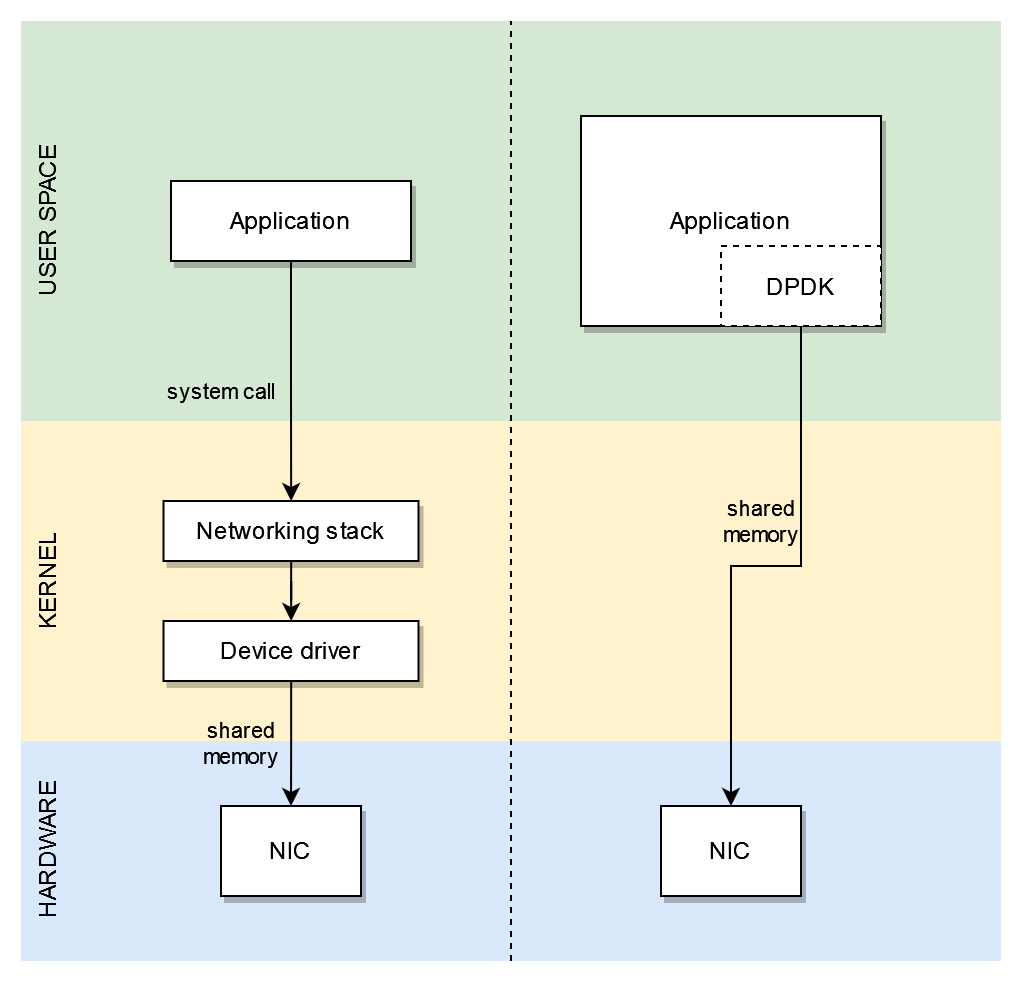
\includegraphics[width=0.7\textwidth]{graphics/trad-vs-dpdk.png}
    \caption{Data path monolitico vs DPDK}
    \label{fig:trad-vs-dpdk}
\end{figure}

Lo scenario descritto è adatto alla maggior parte degli usi: esso consente infatti di non sprecare cicli di clock con attese attive favorendo efficienza, risparmio energetico ed esponendo un'API semplice (le system call) uguale per ogni applicazione. Un elemento di rete però non è fatto per stare a riposo: sulle sue interfacce è logico trovare sempre traffico e deve dunque essere progettato focalizzandosi sulle alte prestazioni. L'alto livello di integrazione e il numero finito di funzioni che esso implementa consentono inoltre di rinunciare a qualche punto di flessibilità in favore delle performance.

Da queste idee è nata DPDK, una libreria per sviluppare applicazioni di networking in grado di gestire efficacemente un throughput molto elevato, nell'ordine di centinaia di Gigabit per secondo. Gli ingredienti fondamentali sono semplici:

\begin{itemize}
    \item Bypassare il kernel, permettendo alla scheda di rete di interagire direttamente con la memoria del processo
    \item Spostare i driver in user space, all'interno della libreria stessa
    \item Superare il modello interrupt-driven
\end{itemize}

La prima grande differenza rispetto all'approccio tradizionale è che in DPDK tutto ruota attorno al \textit{poll-mode driver} (PMD): non si usano gli interrupt in favore di una busy wait di nuovi dati in arrivo. Potrebbe sembrare un controsenso, ma ciò consente di incrementare notevolmente il packet rate poiché non si verificano più context switch legati alla gestione degli interrupt e la pipeline della CPU rimane a regime. Il dispositivo di rete quindi scrive i dati in arrivo direttamente in un'area di memoria precedentemente allocata e fissata (pinned) dal processo, il quale consuma gli stessi senza intermediari. 

Sul piano architetturale, trovano spazio i driver per un sott'insieme selezionato di device supportati, uno strato software di astrazione simile all'\textit{hardware abstraction layer} di tutti i principali sistemi operativi, timer e strutture dati, funzioni per l'accelerazione hardware come crittografia o QoS e poco altro. Questi componenti hanno la funzione di interfacciarsi col dispositivo, uniformandone il funzionamento ad alto livello, ed espletare quei compiti che normalmente ricadono sul kernel.

\begin{figure}[htb]
    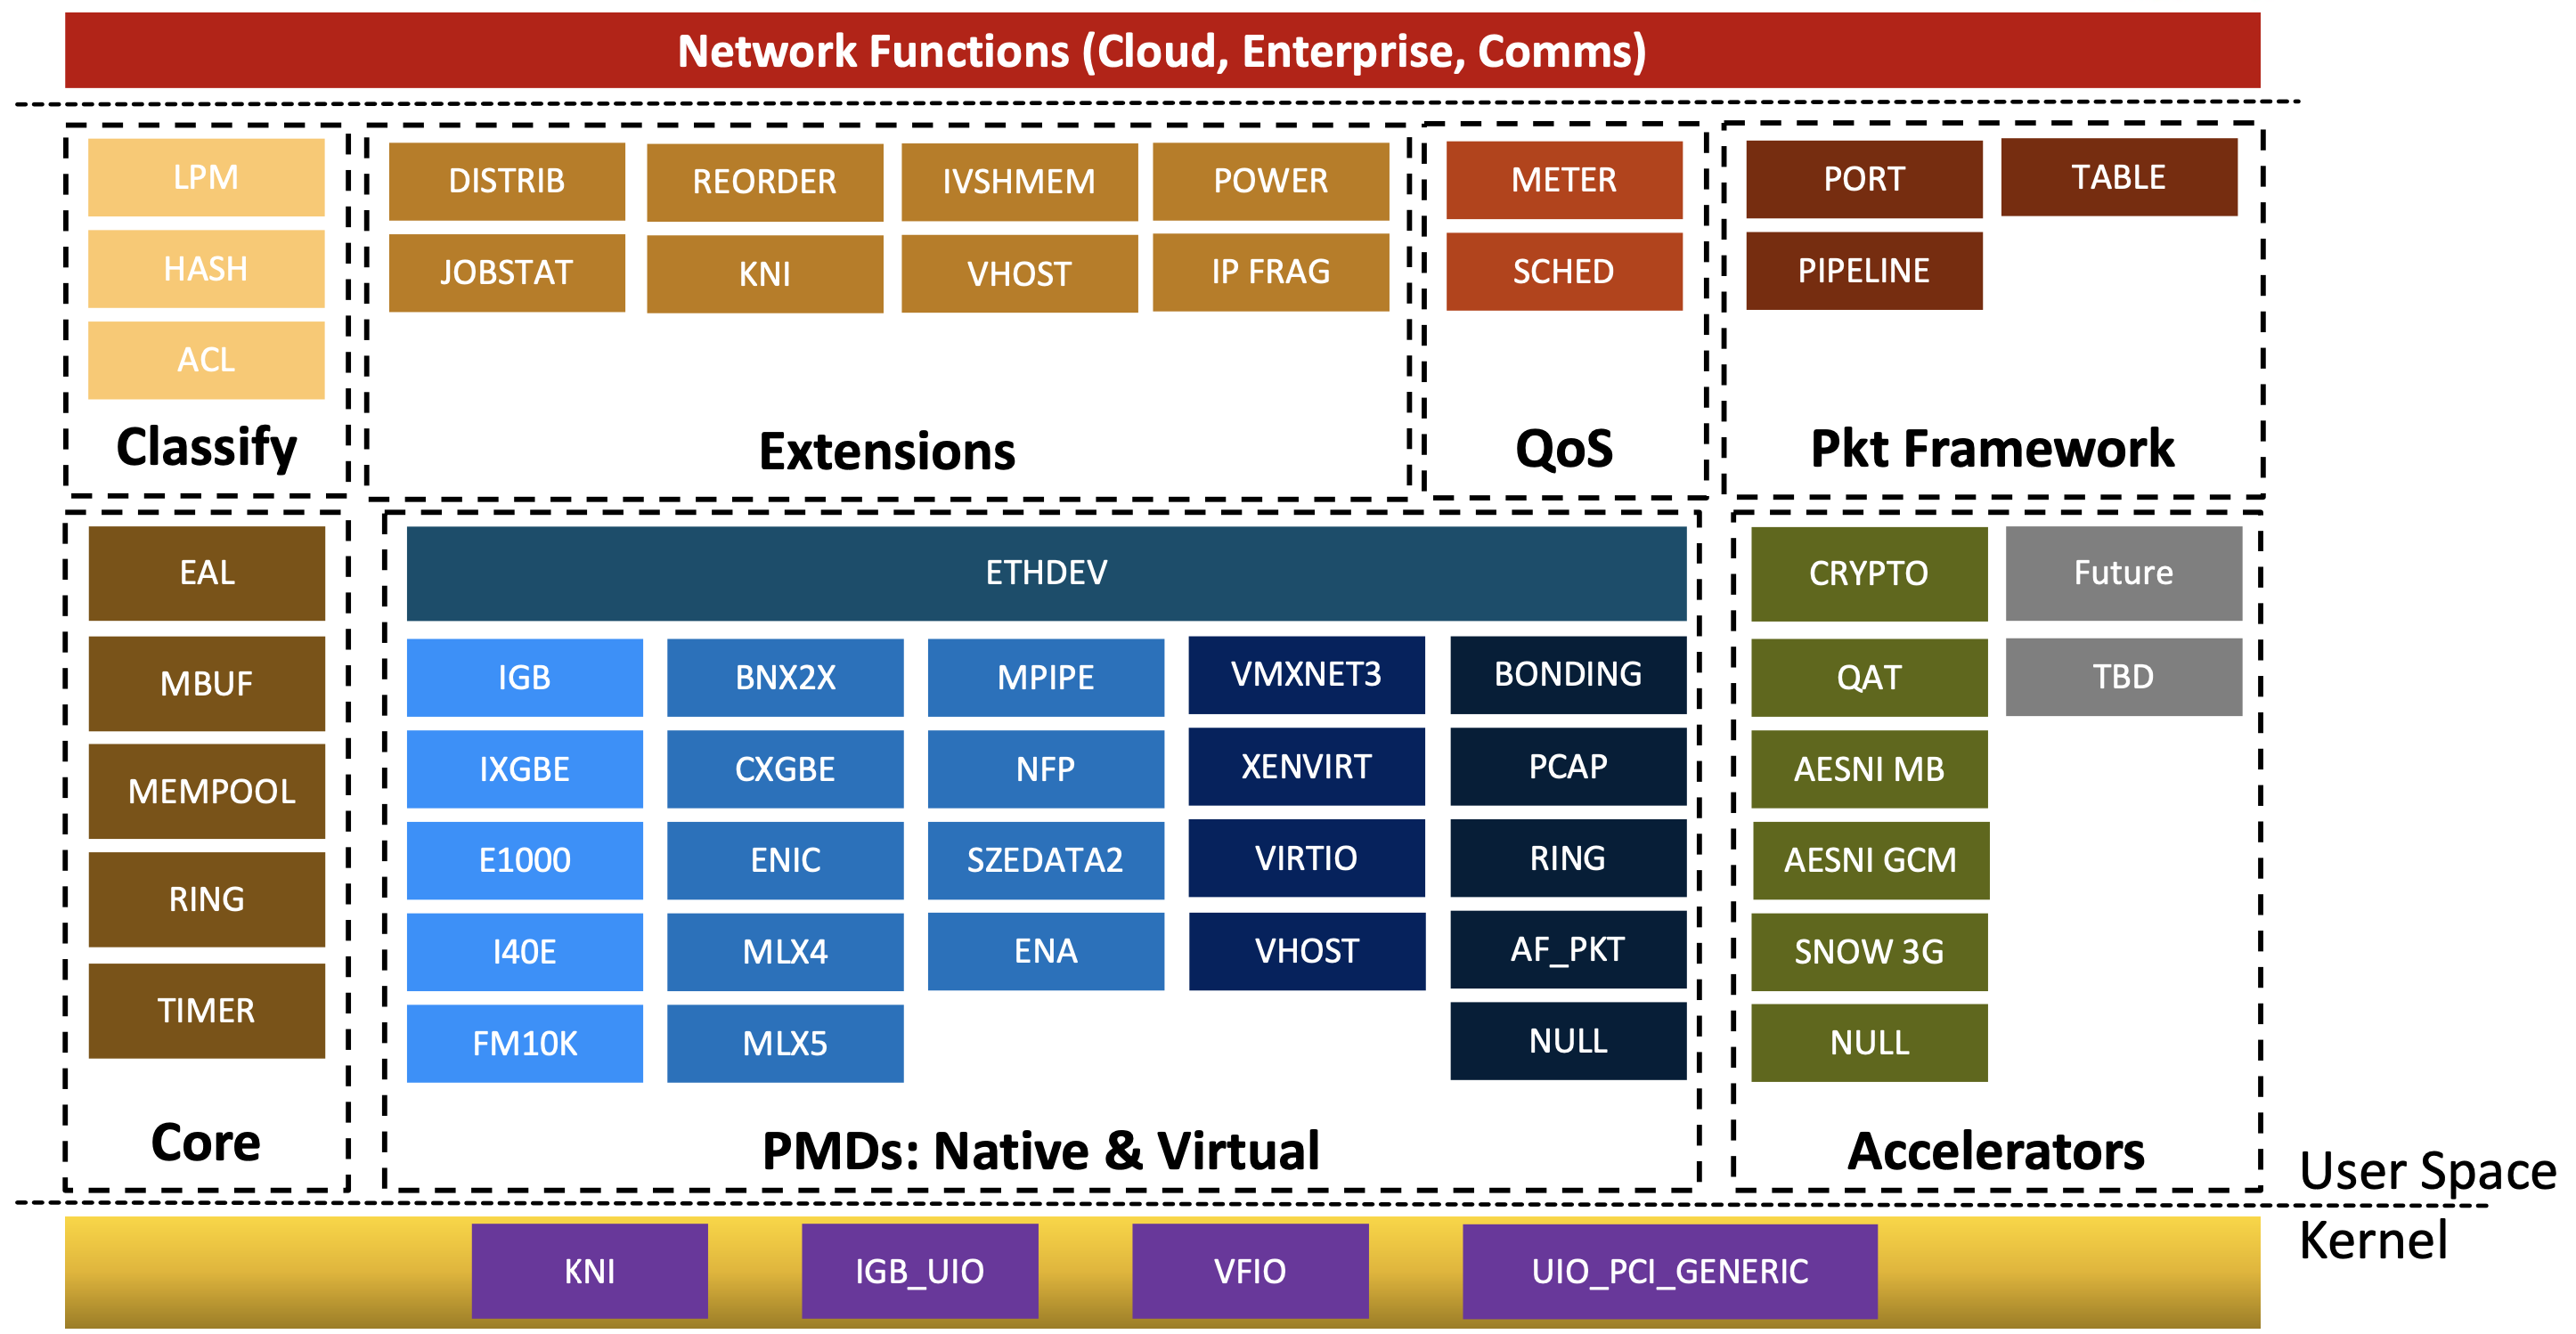
\includegraphics[width=0.8\textwidth]{graphics/dpdk-framework.png}
    \caption{DPDK Framework \cite{dpdk-intro}}
    \label{fig:dpdk-framework}
\end{figure}

Dal punto di vista teorico, DPDK realizza un \textit{exokernel}, ossia una tipologia di sistema operativo in cui il controllo dell'hardware è demandato direttamente ai programmi che ne fanno uso, mentre il nucleo ha la sola funzione di garantire l'accesso esclusivo ai dispositivi da parte dei vari processi. Anche in DPDK infatti quando un'applicazione assume il controllo di un'interfaccia questa diventa non più visibile al resto del sistema.

Nel corso della tesi si illustreranno alcuni usi di questo framework, principalmente legati al routing o al traffic generation, ma DPDK trova spazio anche nelle reti 5G a bassa latenza, nei firewall, in orchestratori come OpenStack o Kubernetes, in ambito HPC e in generale in tutti quei contesti dove il networking ad alte prestazioni è una prerogativa imprescindibile.

\section{VPP}
\label{sec:vpp}

Il paragrafo precedente descrive come DPDK assolva i compiti di un device driver, permettendo al software di dialogare con l'hardware in maniera efficiente grazie all'introduzione del poll-mode driver in user space. Il prossimo tassello dello stack tecnologico è rappresentato dal data plane. Anche in questo caso, trattandosi di un'architettura interamente virtualizzata e senza un particolare supporto hardware dedicato, entra in scena una libreria, frutto del lavoro di Cisco, open source e votata alla velocità.

L'intuizione fondamentale dietro VPP, acronimo di \textit{Vector Packet Processing}, è quella di sfruttare al massimo la pipeline delle moderne CPU scalari, operando su insiemi di dati piuttosto che pacchetti singoli al fine di ottimizzare l'utilizzo delle cache. Analogamente a quanto descritto nel paragrafo su DPDK, i pacchetti devono attraversare una serie di ``stazioni'' durante la loro elaborazione, ciascuna delle quali svolge una funzione precisa, come decodificare un header o interrogare una tabella d'inoltro.

\begin{figure}[htb]
    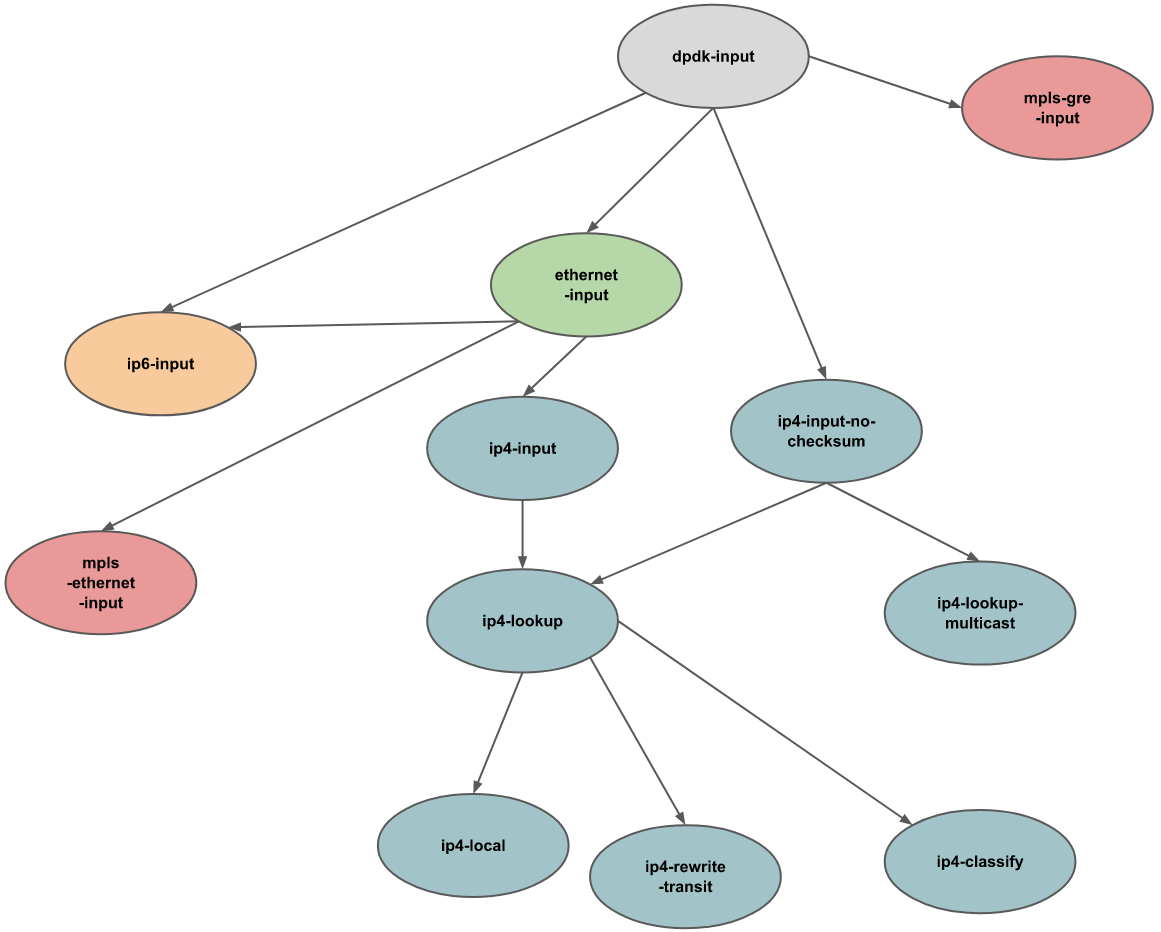
\includegraphics[width=0.7\textwidth]{graphics/vpp-dag.png}
    \caption{Il grafo diretto aciclico di VPP (estratto) \cite{vpp-overview}}
    \label{fig:vpp-dag}
\end{figure}

In VPP queste operazioni sono descritte da un grafo diretto aciclico (DAG) che definisce il flusso dei pacchetti sul data plane. La soluzione di Cisco però si differenzia nell'approccio. Nei sistemi operativi tradizionali, ogni pacchetto attraversa individualmente la pipeline di processing. Sommariamente, questo si traduce nei seguenti passi:

\begin{itemize}
    \item Load del pacchetto dati
    \item Load delle istruzioni inerenti una stazione di elaborazione
    \item Processing vero e proprio
    \item Load delle istruzioni inerenti la successiva stazione di elaborazione
    \item Processing
    \item ...
\end{itemize}

Le operazioni di load in particolare sono onerose in termini di cicli di clock, poiché richiedono importanti trasferimenti dalla memoria. VPP mira a risolvere questa criticità operando su \textit{vettori} di pacchetti piuttosto che singole unità. Se infatti la latenza di memoria dovuta al recupero delle istruzioni è inevitabile, una volta che queste hanno raggiunto la instruction cache della CPU possono essere riapplicate a molteplici dati della stessa natura aumentando l'efficienza in termini di pacchetti per secondo tanto più aumenta la dimensione del vettore. Parallelamente i pacchetti vengono caricati nella data cache in blocco, avvantaggiati dalle funzioni di load speculative delle moderne microarchietture. Applicando simultaneamente queste due ottimizzazioni, si riescono a ridurre significativamente i cache miss sia sulle istruzioni, poiché queste vengono riapplicate in serie per $N$ pacchetti, che sui dati, trasferiti a scaglioni, risultando in un incremento fino a 4-5 volte del numero di pacchetti elaborati al secondo da un singolo core.

Si tratta quindi di rovesciare il punto di vista quando si elaborano i pacchetti ragionando per livelli come meglio chiarito nella \cref{fig:scalar-vs-vector-packet-processing} invece che per unità. Ciò acquista maggior significato se si tiene conto dei pochi compiti in capo al data plane, che al più può incapsulare o decapsulare tunnel di varia natura, inoltrare pacchetti su interfacce diverse e tradurre indirizzi. Inoltre, risiedere in user space permette una sensibile flessibilità in fase di sviluppo e adozione di nuove funzionalità, così come consente un agile recupero in caso di errore: un'applicazione può essere riavviata senza troppi problemi, mentre un eventuale crash del kernel sarebbe catastrofico. Discorso analogo vale per gli aggiornamenti.

\begin{figure}[htb]
    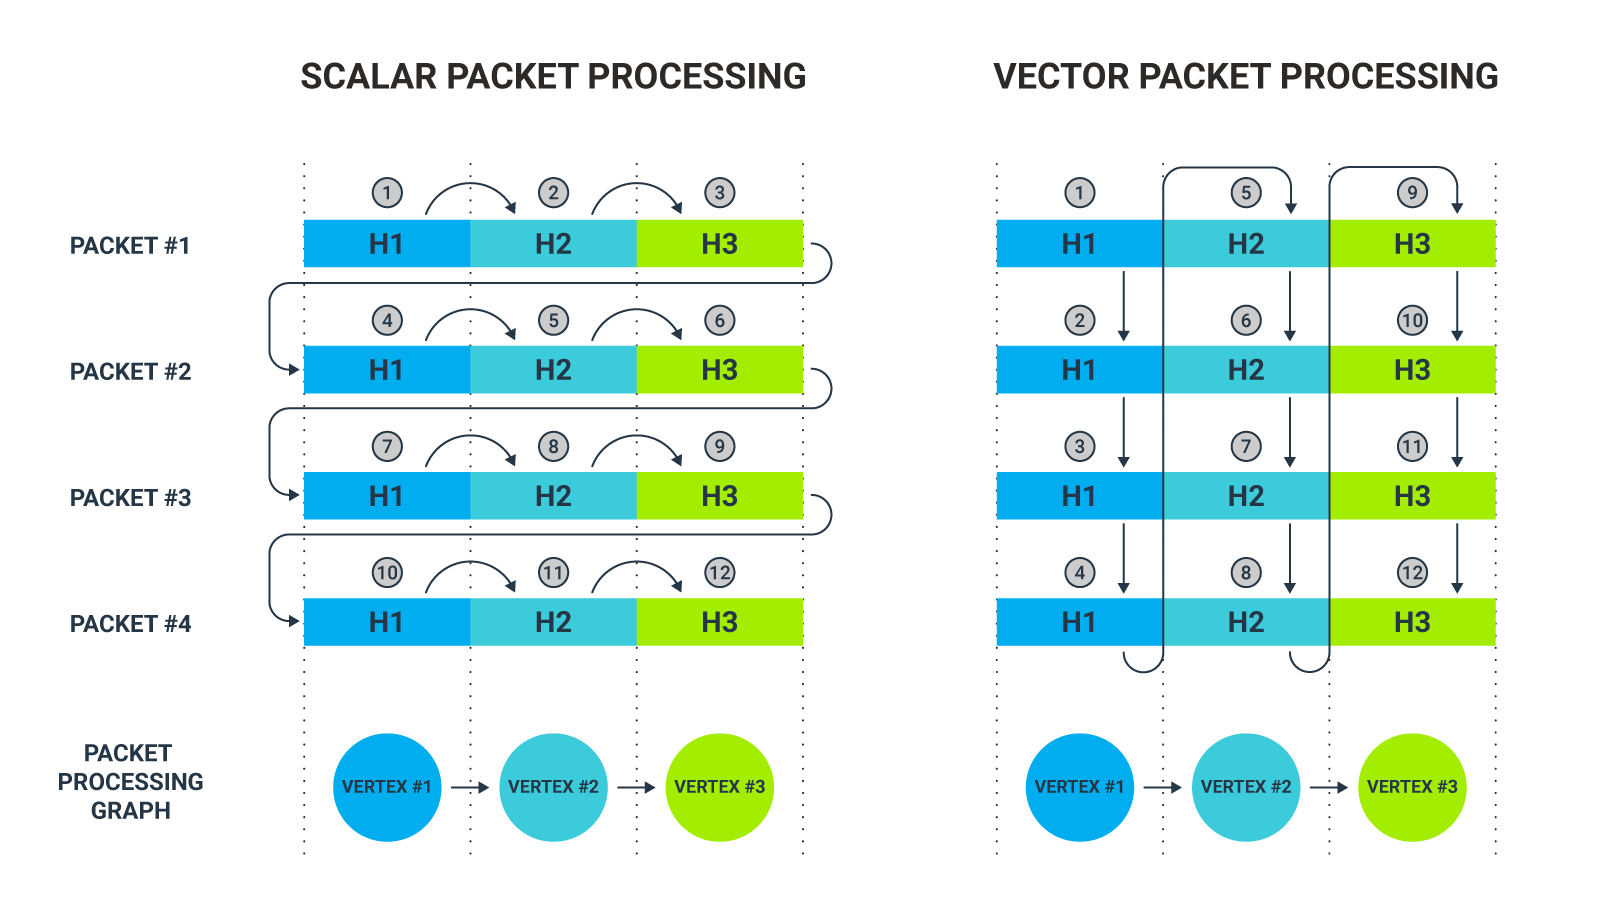
\includegraphics[width=0.8\textwidth]{graphics/codilime_scalar_packet_processing_vs_vector_packet_processing.png}
    \caption{Processing unitario (scalare) vs vettoriale}
    \label{fig:scalar-vs-vector-packet-processing}
\end{figure}

Come DPDK, anche VPP è passato sotto l'ombrello della Linux Foundation confluendo nel \textit{Fast Data Project} (FD.io). A livello architetturale, DPDK costituisce l'input per VPP e spesso quest'ultimo incorpora il primo come dipendenza software nelle vesti di plug-in (v. \cref{fig:vpp-dag} ``dpdk-input''). Trattandosi di componenti software, infine, entrambe si prestano ad applicazioni di vario genere, adattandosi facilmente a molti scenari cloud come macchine virtuali e container.

\section{FRRouting}

DPDK e VPP forniscono quanto necessario per realizzare un data plane software ad alte prestazioni, formando una sorta di ASIC virtuale. Chiave di volta per rendere operativa questa infrastruttura è un control plane in grado di istruire il piano d'inoltro nelle sue funzioni vitali e coordinarsi con gli altri apparati della rete per dirigere il traffico.

Entra dunque in scena \textit{Free Range Routing}, l'ultimo e forse più semplice elemento di questa architettura interamente virtuale. Nato come fork di Quagga, a sua volta derivato dall'ormai abbandonato GNU Zebra, FRRouting è un software libero composto da una collezione di demoni che implementano i più comuni protocolli del control plane oggi utilizzati. Al suo interno troviamo il trittico BGP/OSPF/IS-IS che nelle sue varie declinazioni domina il panorama intra- ed inter- sistemi autonomi, ma anche protocolli dedicati al multicast come PIM e IGMP, LDP per la distribuzione delle etichette MPLS, EVPN ed altri.

\begin{figure}[htb]
    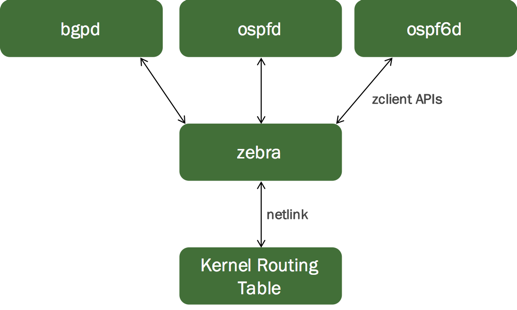
\includegraphics[width=0.7\textwidth]{graphics/frrouting-overview-daemons.png}
    \caption{Architettura di Free Range Routing}
    \label{fig:frr-arch}
\end{figure}

Il design è caratterizzato da una topologia master/slave (\cref{fig:frr-arch}) al cui centro trova spazio il demone principale, \textit{zebra}. Questo svolge il ruolo di accentratore per le informazioni provenienti dalle varie altre entità e si occupa di interfacciarsi col sistema operativo tramite \textit{netlink}, un protocollo di sistema aperto per la gestione delle interfacce di rete e del data plane.

Nei paragrafi precedenti è stato illustrato come DPDK e VPP si siano evoluti seguendo una filosofia bottom-up, ossia costruendo via via gli elementi necessari e astraendo il funzionamento dei livelli sottostanti. FRR invece ha vissuto una storia diversa: affermatosi prima dell'avvento di queste soluzioni innovative, ha sempre vissuto comodamente sopra qualunque tipo di sistema operativo senza richiedere particolari risorse. Sono state proprio la sua completezza e stabilità a renderlo il compendio ideale del panorama virtuale, tanto che nel giro di un paio d'anni sono stati fatti molteplici tentativi per integrarlo con lo strato superiore di VPP\footnote{\ La già citata Southbound API della \cref{sec:sdn-nfv}}. L'ultimo nonché l'unico ad aver avuto abbastanza successo da essere supportato nativamente si chiama \textit{linux-cp}, acronimo di ``Linux Control Plane'', ed è stato descritto dall'autore in una serie di articoli \cite{pim-linux-cp}. Il concetto è semplice: creare un'interfaccia virtuale gemella di quella fisica nel sistema operativo su cui VPP possa riversare tutto il traffico diretto specificatamente al router e mantenerne la configurazione allineata a quella interna. Ciò non costituisce un problema poiché la maggior parte dei pacchetti che attraversano un router sono solitamente ``di passaggio'', senza essere destinati all'apparato stesso, e quindi non lasceranno mai il data plane. I pochi restanti invece possono migrare da un dominio all'altro in maniera trasparente, beneficiando di tutto il software e la logica già comunemente presenti e senza reinventare la ruota.

All'atto pratico, \textit{linux-cp} è anch'esso un plug-in, un nodo del grafo diretto aciclico di VPP, ed è logicamente suddiviso in due parti:

\begin{enumerate}
    \item \textbf{Interface Mirror} che si occupa della sincronizzazione VPP \textrightarrow\ Linux
    \item \textbf{Netlink Listener} il cui compito è rimanere in ascolto dei messaggi \textit{netlink} in arrivo dal livello applicativo e apportare le dovute modifiche alla coppia di interfacce
\end{enumerate}

Grazie a Netlink e a \textit{linux-cp} è possibile collegare FRRouting al data plane evoluto VPP/DPDK (\cref{fig:tnsr-arch}) seguendo una metodologia top-down. Il plug-in permette inoltre di sfruttare tutti i classici strumenti come \textit{ping} e \textit{traceroute} sopra al nuovo stack senza necessità di modifiche.

\section{TNSR}

I tre paragrafi precedenti introducono i pilastri del routing interamente softwarizzato, di cui rappresentano lo stato dell'arte. Combinarli però non è banale: si rischiano incompatibilità e colli di bottiglia difficili da scovare. Per questo motivo Netgate ha creato TNSR, una distribuzione di Linux basata su Ubuntu\footnote{\ Precedentemente si basava su CentOS, con differenze minime} che presenta un ambiente preconfigurato simile ad un router commerciale. L'azienda, già famosa per aver creato pfSense, un firewall virtuale open source molto apprezzato, è impegnata nel contribuire all'ecosistema con l'obiettivo di rafforzarlo e renderlo più adatto ad un uso reale, intravedendo in TNSR uno step intermedio verso un firewall ad alte prestazioni.

Peculiarità di TNSR è la suddivisione in namespace. Linux mette a disposizione questa tecnologia per favorire l'isolamento dei processi e delle risorse, di fatto la base della cosiddetta ``OS-level virtualization'', comunemente nota come \textit{container}. Nella fattispecie, TNSR usa due distinti networking namespaces per il router ed il management plane: il primo, chiamato ``dataplane'', contiene lo stack VPP/DPDK, la suite FRR e Strongswan per la gestione dei tunnel IPSec, mentre nel secondo si trovano la CLI, il server SSH per l'accesso remoto, il database delle configurazioni e altri strumenti utili alla gestione del router e del suo sistema operativo.

\begin{figure}[htb]
    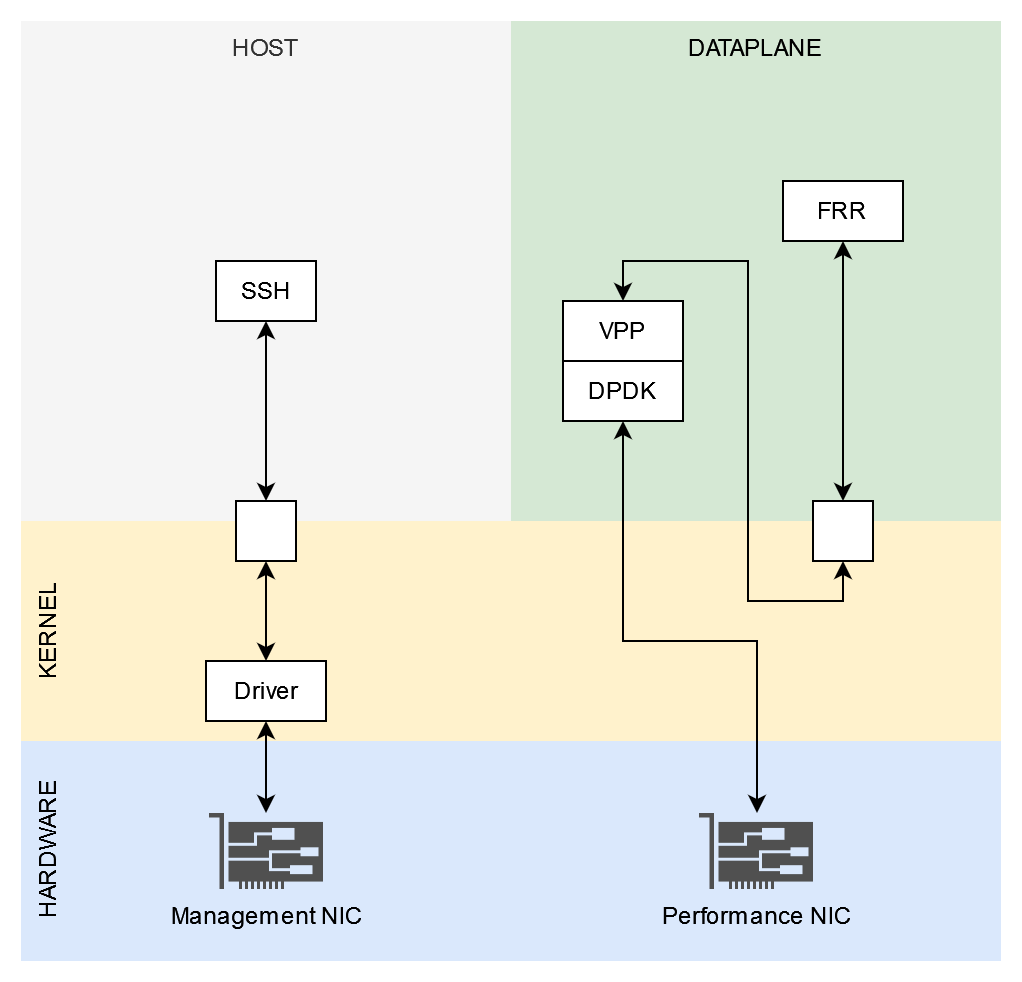
\includegraphics[width=0.7\textwidth]{graphics/tnsr-arch.png}
    \caption{Architettura di TNSR (estratto)}
    \label{fig:tnsr-arch}
\end{figure}

Separare i due ambienti in questo modo offre svariati vantaggi: in primo luogo previene che malfunzionamenti in una o nell'altra parte possano ripercuotersi sull'operatività generale del router, potendo ad esempio disporre di un'entrata di management anche in caso di errori di configurazione del dataplane. Inoltre, siccome i dispositivi di rete così come i processi sono isolati all'interno di ciascun namespace, non si rischia confusione durante l'assegnazione delle interfacce che possono essere acquisite automaticamente dai rispettivi stack di rete. Anche le tabelle di inoltro sono diverse, fattore che contribuisce alla sicurezza generale e all'affidabilità della soluzione. Ultimo ma non meno importante, testimonia come queste tecnologie possano funzionare all'interno di container, caratteristica che ne aumenta l'appetibilità col passare del tempo. Non sorprenderebbe se in futuro questi software raggiungessero un livello di maturità tale da essere orchestrati su cluster di container all'edge della rete. Oggi tuttavia la tecnologia è ancora acerba: manca ad esempio la possibilità in orchestratori come Kubernetes di definire la presenza di una certa scheda di rete come requisito. Alcuni plug-in promettono di estenderne le funzionalità, ma non sembrano attrarre particolare interesse, almeno per il momento. Virtualizzatori come Proxmox, invece, già consentono di eseguire container al pari di macchine virtuali, ma così facendo verrebbe meno la parte di resilienza, fallback e load balancing automatici.

È opinione di chi scrive che la semplice architettura di TNSR, elegante e funzionale, tornerà a far parlare di sé in futuro, venendo rivisitata in altre applicazioni simili per mezzi, ma diverse per finalità.

% https://m.facebook.com/NetgateUS/posts/10155790595267689

\section{DANOS}

Finora si è parlato di stack completamente virtuali, senza l'ausilio di acceleratori hardware legati a funzionalità specifiche. Questo approccio è generalmente preferibile quando si ha a che fare con funzioni diverse e complesse quali ad esempio certe componenti dell'architettura LTE. Nel caso del puro forwarding invece è difficile raggiungere throughput importanti senza circuiti dedicati: nonostante molti studi e gli esperimenti che verrano discussi nel \cref{chap:lab} suggeriscano che la suite VPP/DPDK scali linearmente all'aumentare della potenza di calcolo, permangono limiti fisici, tecnologici ed economici che ne scoraggiano l'utilizzo in condizioni di traffico molto elevato come la rete core di un grande provider.

Queste ragioni hanno guidato lo sviluppo di una nuova classe di dispositivi, i \textit{whitelabel switch}. Si tratta in sostanza di router e switch simili agli apparati tradizionali, ma privi di sistema operativo. A realizzarli sono spesso aziende nuove del settore, case come Broadcom, specializzata in chip, che decidono di cimentarsi nell'impresa di produrre processori dedicati, chiamati \textit{network processing unit} o più sovente \textit{merchant silicon}, e di venderli ad altre realtà affinché possano produrre soluzioni complete. Diversamente dai vendor verticalmente integrati, questa famiglia è caratterizzata da ASIC programmabili e quindi facilmente customizzabili tanto che si stanno affermando nuovi linguaggi di programmazione specificatamente orientati all'implementazione di nuovi protocolli del data plane, tra cui \textit{P4}.

DANOS è un sistema operativo disaggregato e aperto per apparati di rete \cite{danos-whitepaper}. Il suo obiettivo non è realizzare una soluzione completamente softwarizzata, ma piuttosto di essere in grado di dialogare con qualunque tipo di data plane, fisico o virtuale. Contiene dunque al suo interno i driver necessari ad interfacciarsi con l'hardware specializzato sottostante per l'offload di task specifici realizzando di fatto una Southbound API verso il \textit{merchant silicon}. Anche il control plane nasce con l'intento di essere modulare, potendo spaziare da un edge router ad un gateway per la telefonia mobile.

Il progetto è ancora acerbo, l'immagine aperta pubblicata contiene un data plane basato su DPDK e derivato da quello di Vyatta, un altro famoso router virtuale costruito su Linux. Vista la natura sperimentale, è probabile che alcune grandi aziende ne usino internamente versioni customizzate per i propri fini. Dal 2018 è entrato a far parte anch'esso della Linux Foundation, ma la community è poco attiva e l'entusiasmo iniziale sembra scemato. Forse in futuro, col progresso della tecnologia e dei whitelabel switch, se ne sentirà di nuovo parlare, ma resta un buon esempio delle molteplici iniziative di networking aperte ed interoperabili nonché dei diversi approcci saggiabili nel settore.

\section{XDP}

Parallelamente alla nascita di DPDK, altre tecnologie vedevano la luce tra cui \textit{eXpress Data Path} (XDP): una ``scorciatoia'' nel kernel Linux introdotta nella versione 4.8 \cite{xdp-paper}. Nei paragrafi precedenti si è discusso come DPDK scelga la strada radicale di bypassare in toto il kernel, spostando tutto il processing in user space; al contrario XDP è più conservativo e si avvale di un filtro programmabile insito in Linux per effettuare alcune operazioni ``al volo'' prima che i pacchetti lascino il driver, prima ancora che il sistema operativo allochi i buffer necessari a contenerli.

Grazie una macchina virtuale chiamata \textit{extended Berkeley Packet Filter} (eBPF) e supportata dalla maggior parte dei driver di rete\footnote{\ Talvolta pure a bordo delle stesse NIC in modalità offload} è possibile scrivere un programma, sicuro by design, che prenda decisione sulla base di campi prefissati del pacchetto ed esegua alcune semplici azioni come:

\begin{itemize}
    \item \verb|DROP|, per scartare il pacchetto
    \item \verb|TX|, per ritrasmettre il pacchetto alla stessa scheda che l'ha ricevuto, eventualmente dopo averlo modificato
    \item \verb|REDIRECT|, per spostare il pacchetto su un'altra NIC o inviarlo ad un programma in user space tramite un socket \verb|AF_XDP|
    \item \verb|PASS|, per continuare la classica pipeline di elaborazione
\end{itemize}

\begin{figure}[htb]
    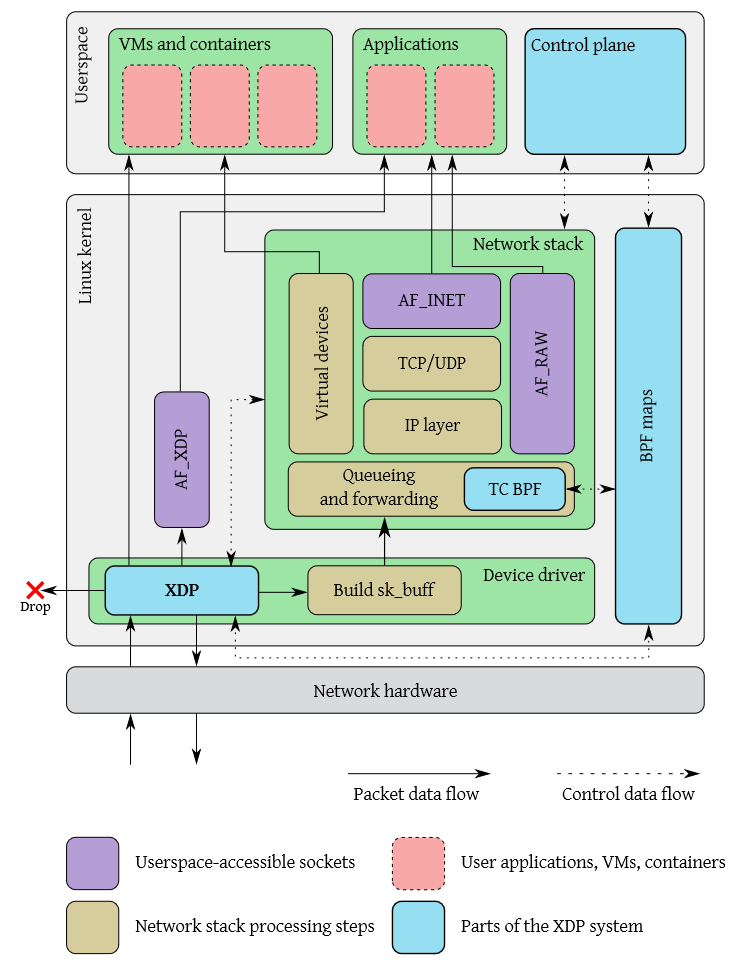
\includegraphics[width=0.7\textwidth]{graphics/xdp-datapath.png}
    \caption{Anatomia di XDP}
    \label{fig:xdp-datapath}
\end{figure}

Gli usi sono molteplici: la possibilità di passare i pacchetti allo user space o a delle macchine virtuali consente di implementare una funzione simile a quella dei controllori SDN per il traffico non classificato. Si può inoltre realizzare un router, tenendo però a mente che eventuali regole di firewall andrebbero reimplementate, in quanto normalmente situate più a valle nella pipeline di processing \cite{xdp-router-apnic}. In alternativa, questo tipo di filtro si presta molto bene alla mitigazione di attacchi di tipo DDoS, alleggerendo il sistema operativo dall'overhead dovuto al processing dei pacchetti malevoli \cite{cloudflare-ddos-xdp}.

Sul piano delle performance non può beneficiare dei vantaggi ``vettoriali'' di VPP, ma riesce ugualmente ad ottenere risultati sensibilmente superiori all'elaborazione tradizionale. Un altro tallone d'Achille è l'intrinseca limitazione: a partire da Linux 5.1 i programmi XDP sono limitati ad eseguire un milione di istruzioni\footnote{\ Prima erano solamente 4096!}, non potendo quindi ambire a task più complessi di un router o di un semplice packet filter.

\section{TRex}

Delle tante applicazioni di DPDK, una sicuramente degna di nota è TRex, un traffic generator L3-7 open source creato da Cisco. A differenza di altri prodotti commerciali, TRex non punta a creare traffico ex novo, ma si limita a replicare dei flussi di catture esistenti modificando i campi chiave dei pacchetti e potendo contare sull'alta efficienza di DPDK per invio e ricezione. Questa combinazione permette di raggiungere velocità nell'ordine di centinaia di Gigabit al secondo su un moderno laptop, abbattendo sensibilmente i costi legati a questo tipo di appliance. Il software presenta due principali modalità operative:

\begin{itemize}
    \item Stateless, adatto a testare apparati di livello 3 e tunnel, supporta fino a \mbox{10mila} stream paralleli e 30 milioni di pacchetti al secondo per core e permette di misurare latenza e jitter dei pacchetti
    \item Stateful, in grado di emulare un protocollo livello 7, ottimo per mettere alla prova NAT, firewall, load balancer ed altri applicativi che si avvalgono della cosiddetta \textit{Deep Packet Inspection} (DPI)
\end{itemize}

A livello hardware, supporta tutte le schede di rete supportate da DPDK, \eng{device} virtualizzati, SR-IOV ed è possibile eseguirlo dentro un container. Ovviamente, perché raggiunga il massimo delle potenzialità, sono necessarie alcune accortezze legate al discorso NUMA che verranno meglio affrontate nel \cref{chap:lab}, ma tramite la configurazione guidata molti passaggi vengono espletati in automatico.